\documentclass{article}
\usepackage{../FinalYearProjectReport}

% packages for apendicies
\usepackage{color}
\usepackage{listings}
\definecolor{gray}{rgb}{0.4,0.4,0.4}
\definecolor{darkblue}{rgb}{0.0,0.0,0.6}
\definecolor{cyan}{rgb}{0.0,0.6,0.6}

\lstset{
  basicstyle=\ttfamily,
  numbers=left,
  columns=fullflexible,
  showstringspaces=false,
  commentstyle=\color{gray}\upshape
}
\lstdefinelanguage{XML}
{
  morestring=[b]",
  morestring=[s]{>}{<},
  morecomment=[s]{<?}{?>},
  stringstyle=\color{black},
  identifierstyle=\color{darkblue},
  keywordstyle=\color{cyan},
  morekeywords={xmlns,version,type}% list your attributes here
}
\lstdefinelanguage{JavaScript}{
  keywords={typeof, new, true, false, catch, function, return, null, catch, switch, var, if, in, while, do, else, case, break},
  keywordstyle=\color{blue}\bfseries,
  ndkeywords={class, export, boolean, throw, implements, import, this},
  ndkeywordstyle=\color{darkgray}\bfseries,
  identifierstyle=\color{black},
  sensitive=false,
  comment=[l]{//},
  morecomment=[s]{/*}{*/},
  commentstyle=\color{purple}\ttfamily,
  stringstyle=\color{darkblue}\ttfamily,
  morestring=[b]',
  morestring=[b]"
}

% packages for references
\usepackage{cite}
\usepackage{url}


% uncomment this line to double line spacing for proof reading
% \linespread{2}

% packages and settings for graphics
\usepackage{float}
\usepackage[pdftex]{graphicx}
\graphicspath{{./images}}
\DeclareGraphicsExtensions{.png}
\usepackage[final]{pdfpages}


\title{Event Syndication and Dissemination}
\name{Chris Morgan}
\address{Department of Electrical and Computer Engineering\\
University of Auckland, Auckland, New Zealand}


\hyphenation{and-roid}


\begin{document}

\begin{titlepage}


\vspace*{15em}


\centering

{\LARGE Department of Electrical and Computer Engineering\\
Part IV Research Project Report\\
2015}

{\LARGE Event Syndication and Dissemination}

\hspace{2em}

% notes on latex tables use "&" as colum sperator
\begin{table*}[h]
\centering
\begin{tabular}{ll}
Project Title: & Event Syndication and Dissemination \\
Project Number: & 2 \\
Supervisor Name: & Sathiamoorthy Manoharan \\
Second Examiner Name: & Gerald Weber \\
Your Name: & Chris Morgan \\
Your UID: & 1744263 \\
Partner Name: & Matthew Dyer \\
Date submitted: & \today \\

\end{tabular}
\end{table*}
\begin{table}


\end{table}
\pagebreak

\vspace*{25em}

{\Large Declaration of Originality}

\hspace{5em}

This report is my own unaided work and was not copied from 
nor written in collaboration with any other person.

Name: Chris Morgan 


\end{titlepage}

\maketitle

\begin{abstract}

\end{abstract}


\section{Introduction}
The state of conference, convention and summit schedules are scattered. The format they come in is inconsistent, either a pdf, mobile application or website. These schedules are often poorly executed and leave a lot of room for improvement. This project will propose a standard schema for such events and deliver example applications to consume event information compliant with the schema. Conference organisers will be able to use this schema to create schedules that can be viewed and navigated on a diverse range of platforms.

There is a need for not only completeness, but also simplicity and usability when designing the schema. It should be as compliant as possible with existing and future conferences while not

\section{Event Schedules Today}
Event schedules come in a variety of formats; pdfs, mobile applications and websites. Event's like Google IO\cite{googleIO2015}, Embedded Linux Conference\cite{embeddedlinuxconference2015} and Apple WWDC\cite{apple2014wwdc} do it right. They provide an easy platform for attendees to find events, plan their schedules and receive updates. However, there are many events that fall short of providing good schedules. For example, IEEE conference schedules \cite{ieeeIMC2014,ieeePSC2015,ieeeICC2014} leave a lot to be desired.

\section{XML vs. JSON}
Choosing a technology to represent the proposed schema required research into industry standards, trends in web technologies as well as standard library support in a multitude of languages. We looked into three candidates JSON (JavaScript Object Notation), XML (eXtensible Markup Language) and OWL (Web Ontology Language). I this report, OWL will not be covered as Matthew did the research on it and semantic web technologies.

\subsection{XML}
When we started this project, XML was the technology that our supervisor recommended we use. It's understandable that it should be the obvious choice, as it is the most widely used resource type in APIs\cite{maleshkova2010investigating}. XML is mature language, first released in 1996 and is used extensively by Microsoft and integrates well into .Net and Java applications.

XSD (XML Schema Definition) is the language used to describe XML schemas and is what would have been used if XML was chosen. The XSD, like most schema definition languages enables the creation of data types, inheritance and validation of data. One of the main inspirations of this project, RSS (Rich Site Summary or Really Simple Syndication) is defined using XSD along with many other XML based data transfer specifications.

\subsection{JSON}
Over the last few years, use of JSON in transferring over the internet and storing data as been increasing in popularity as seen in figure~\ref{fig:JSON_XML_all_time}. Not only this, but new services offering XML are decreasing as shown in figure~\ref{fig:JSON_XML_jan_2013}.

\begin{figure}[h]
	\centering
	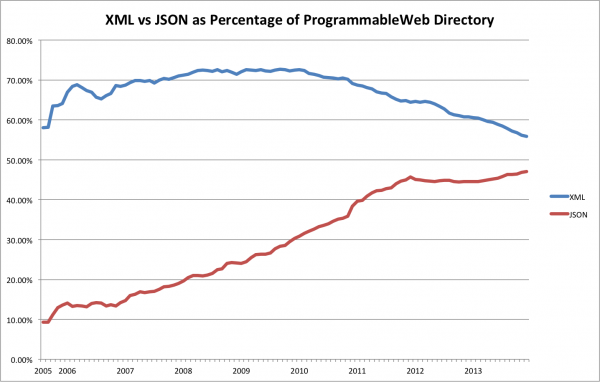
\includegraphics[scale=0.37]{images/xml_json_all_time.png}
	\caption{Overall XML vs. JSON Usage\protect\cite{duvander2013json}}
	\label{fig:JSON_XML_all_time}
\end{figure}

\begin{figure}[h]
  \centering
  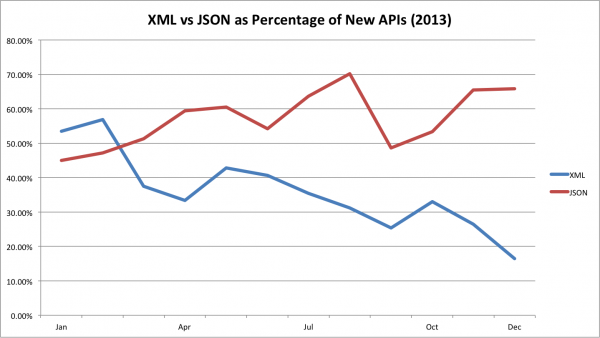
\includegraphics[scale=0.37]{images/xml_json_jan_2013.png}
  \caption{January 2013 New XML vs. JSON Usage\protect\cite{duvander2013json}}
  \label{fig:JSON_XML_jan_2013}
\end{figure}

This is in part due to the increase in the usage of front end web application frameworks such as React, AngularJS, Ember.js and Backbone.js. As such, this shift in usage is no surprise as JSON is easier, faster and cleaner \cite{hellstrom2012querying,lin2012comparison,nurseitov2009comparison} to work with using it's namesake, JavaScript rather than XML. As one of the primary outcomes of this project is to create an example web application, this ease of use plays heavily when choosing which technology to use.

Defining a schema that utilises JSON is not straight forward. As of this report, there is no JSON equivalent of JSON. However, JSON Schema \cite{galiegue2013json} is currently a work in progress specification. Draft 4 has been out for a few years and contains everything necessary to define a JSON schema that can describe conference events. Even though this it is still in draft, with third party library support in many languages \cite{galiegue2013inplementations} and having been unchanged in 2 years it is sufficiently mature to use in a university project.

\subsection{Moving forward}
JSON schema was chosen with modern web technology in mind, as well as wanting to explore emergent technologies. Simply using the de facto technology does not harbour growth, it merely reinforces past experience and research.

\section{Defining a schema}
The first stage of the project was developing a schema to encapsulate conference information. We looked at a multitude of conference schedules as well as mobile applications to understand the scope of what our schema would need to contain.

See listing~\ref{lst:jsonSchema} on page~\pageref{lst:jsonSchema} for the preliminary schema definition. The proposed schema has room for improvement but contains the basic information needed to navigate a conference. Matthew focused more on what should be in the schema while I focused on the technology behind the schema.

\section{Evaluation}
Drafting an event syndication schema and implementing consuming applications is all well and good, however validating the quality, usability and completeness of what was done requires objective evaluation. Conference schedules already exist, this project isn't trying to change how they are structured or determined but rather provide a compliant data format for organisers to utilise in order to distribute schedule information.

To evaluate the outcome of this project, conferences from in a variety of formats and structures will be translated into the proposed schema. If conference information is unable to be translated to fit the schema, that would weigh negatively, while ease of use of the schema would weight positively.

\section{Future work}
The next stage of the project is refining the schema such that it fits with as many conferences as possible without sacrificing excessive amounts of usability. To do this, IEEE conferences will be examined as well as large technology conferences.

In the next few months, we will be implementing 3 separate but similar applications. Initially, we will be developing a web application to consume conference data conforming to the proposed schema. This application will serve as a base for iOS and Android applications. It is planned that we will collaborate on the creation of the web application and then split of on platform native implementations. Matthew will create the Android application and I, the iOS application.

\section{Conclusion}
While current formats of conference information is fractured, the schema this report proposes is a means to standardise how this information is stored and transferred.

\bibliographystyle{IEEEtran}
\bibliography{interim_report}

\onecolumn
\appendix
\section{Schema}
% \lstinputlisting[caption=XML Schema Description, language=XML]{../schema/esad.xsd}
\lstinputlisting[caption=JSON Schema Description, language=JavaScript, label={lst:jsonSchema}]{../../schema/esad.schema.json}


\end{document}